\section{Resultados}

\subsection{Técnicas de procesamiento de imágenes para extraer características relevantes y mejorar la capacidad del modelo de Machine Learning en el reconocimiento y detección de las plagas Stenoma catenifer y heilipus lauri en el cultivo de aguacate Hass a partir de imágenes capturadas en campo.}

\subsubsection{Exploración de datos}

El análisis exploratorio de datos partió de las 744 fotografía del cultivo de aguacate Hass con las cuales se reveló información valiosa sobre la distribución y características de las imágenes. Al examinar la distribución, se observa dos parámetros en la información, el primero corresponde a las imágenes que no presentan el impacto de las plagas (50 imágenes) y el segundo las imágenes que evidencian el proceso de la plaga en el cultivo (694 imágenes). Esto sugiere la necesidad de técnicas de pre-procesamiento para normalizar la información antes de cualquier análisis.

Por esta razón, se estableció dos carpetas de información donde una de ellas se consignan las fotografías que presentan las características de las plantas sana y en la otra carpeta se encuentran las fotografías que muestran las tipologías del impacto de las plagas.

En este sentido, se desarrollaron algoritmos de extracción de características, como por ejemplo el histograma de colores, descriptores de texturas y las características basadas en formas, con las cuales se representa la información relevante de las imágenes dentro del cultivo, para que estas características se conviertan en entradas de reconocimiento en el modelo de aprendizaje automático.

El código en Python está diseñado para la visualización de imágenes de cultivos de aguacate Hass\footnote{El código para la extracción de características de las imágenes se encuentra en GitHub \href{https://github.com/juferoto/mlops_project/blob/master/notebooks/analisisExploratorio.ipynb}{aquí}}, clasificadas en dos categorías: ``Con Plaga'' y ``Sin Plaga''. Este programa, destinado a ser ejecutado en un entorno de Jupyter Notebook, su función principal es cargar y mostrar de manera detallada las dos tipologías definidas en las carpetas con imágenes de cada categoría, permitiendo una inspección visual clara de las características distintivas entre los cultivos afectados por plagas y aquellos que se consideran saludables.

\newpage

\begin{figure}[h]
\centering
\caption{Exploración de datos}
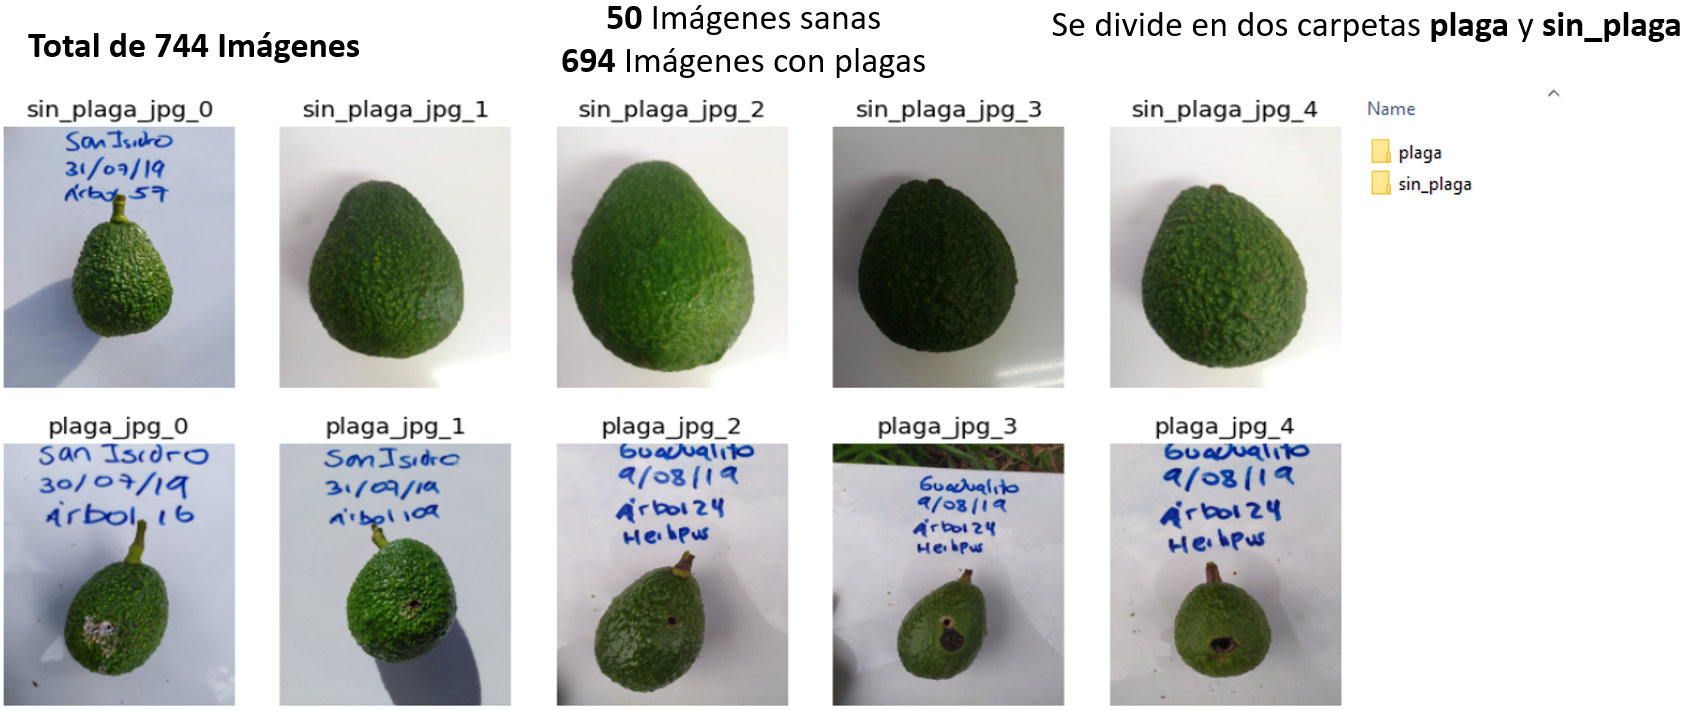
\includegraphics[width=0.8\textwidth]{resultados/expDatos.png}
\caption*{\footnotesize Fuente: Elaboración Propia}
\label{fig:figuraExpDatos}
\end{figure}

Al realizar un análisis exploratorio de datos para comprender la distribución y características de las imágenes se puede señalar que, las imágenes sin plagas corresponden al 6,72\% y las imágenes con plagas el 93,28\% como se describe a continuación:

\begin{figure}[h]
\centering
\caption{Distribución porcentual de las categorías de las imágenes}
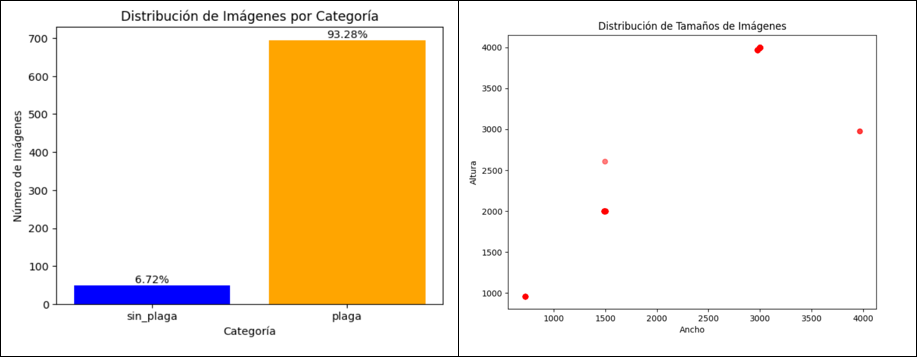
\includegraphics[width=0.6\textwidth]{resultados/distPorcentual.png}
\caption*{\footnotesize Fuente: Elaboración Propia}
\label{fig:figuraDistPorcentual}
\end{figure}

Se puede decir que las imágenes que generan mayor información corresponden a las que tienen plagas. Asimismo, la distribución de tamaño de imagen se observa que, identifican imágenes con un ancho de 4.000 píxeles por 3.000 píxeles de altura o por el contrario 3.000 de ancho por 4.000 de altura, donde se tomaron las fotografías tanto verticales como horizontales manteniendo esa rotación.

\newpage

Por lo tanto, se generó el código correspondiente para generar tanto la distribución de imágenes por categoría como la distribución por tamaños, y por otro lado, se generó un código para saber cómo está distribuido por cada alto y ancho de las imágenes. 

Como se puede ver en la imagen que el 87,6\% de las imágenes presentan una resolución de 4.000 píxeles por ancho y por el lado de las alturas más del 87,6\% tienen 3000 píxeles de alto \footnote{El código para el tratamiento de imágenes por categoría y alturas se encuentra en GitHub \href{https://github.com/juferoto/mlops_project/blob/master/notebooks/analisisExploratorio.ipynb}{aquí}}.

\begin{figure}[h]
\centering
\caption{Distribución alto y ancho de las imágenes}
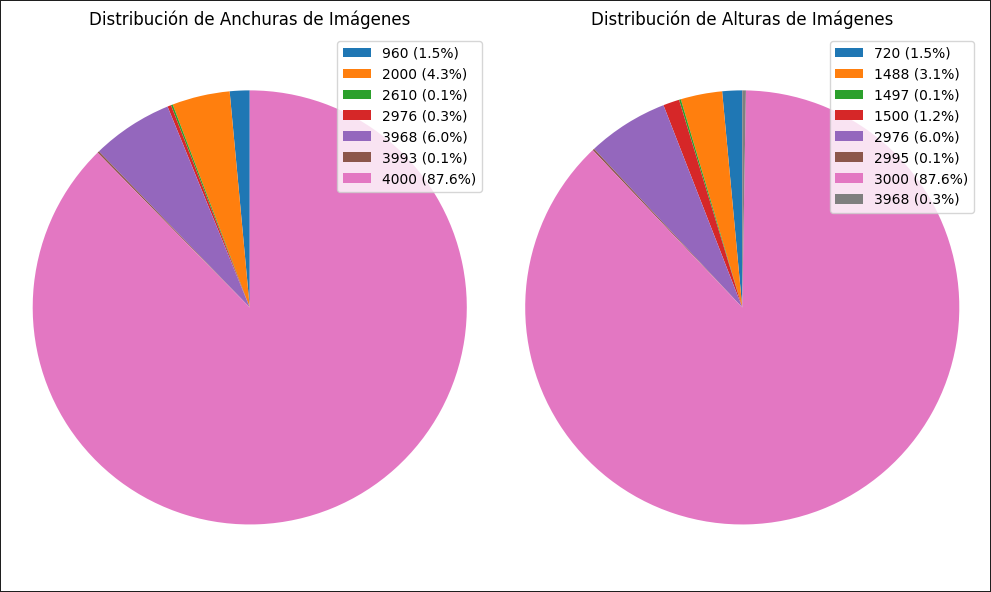
\includegraphics[width=0.7\textwidth]{resultados/distAlturas.png}
\caption*{\footnotesize Fuente: Elaboración Propia}
\label{fig:figuraDistAlturas}
\end{figure}

\subsubsection{Remoción de fondo de imagen}

Quitar el fondo de cada una de las imágenes dejando solo el aguacate, enfocándose solamente en las imágenes que muestra signos de plagas, es esencial en el análisis de las imágenes para la detección y monitoreo de enfermedades. Al aislar el aguacate de su entorno, se simplifica la tarea de identificación de posibles plagas y enfermedades, permitiendo una evaluación más precisa y eficiente\footnote{El código de eliminación de fondo de las imágenes se encuentra en GitHub \href{https://github.com/juferoto/mlops_project/blob/master/notebooks/removerFondo.ipynb}{aquí}}.

\newpage

Este enfoque mejora la capacidad de los algoritmos de visión para identificar patrones sutiles asociados con enfermedades específicas, ya que elimina distracciones no relevantes y optimiza la focalización en las características de interés.

Todas las 744 imágenes presentaban un fondo que podría introducir ruido durante el análisis. Por lo tanto, se llevó a cabo el proceso para eliminar las imágenes del fondo, dejándolas libres de ruido. El resultado final consiste en la preservación únicamente de la parte central de la imagen, como se aprecia en la imagen anterior con el código implementado realiza la tarea de eliminar el fondo y retener solo la imagen del aguacate.

\begin{figure}[h]
\centering
\caption{Proceso de remoción de fondo de las imágenes}
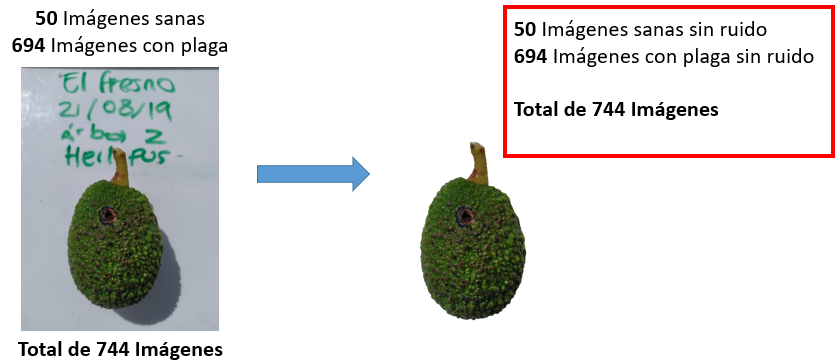
\includegraphics[width=8cm]{resultados/remFondo.png}
\caption*{\footnotesize Fuente: Elaboración Propia}
\label{fig:figuraRemFondo}
\end{figure} 

La efectividad de este código asegura que las imágenes estén listas para ser utilizadas en análisis más detallados y precisos relacionados con el aguacate y cualquier aspecto asociado, sin la interferencia de fondos indeseados.

\subsubsection{Procesamiento de imágenes}

En el procesamiento de la segmentación de imágenes como se viene señalando en los anteriores momentos, permite resaltar la zona en donde se encuentra las caracteristicas propias de la plaga. El proceso tiene como fin facilitarle al algoritmo de Machine learning interpretar las imágenes. Este enfoque se integra en la fase de pre-procesamiento para resaltar la zona afectada por la plaga, simplificando la tarea del algoritmo y mejorando su capacidad de interpretación.

A cada una de estas 694 imágenes que presentan afectaciones de la plaga se trazó un polígono para saber en dónde estaba ubicada la plaga, este polígono genera unas coordenadas que luego van a ser interpretadas por uno de los algoritmos usados para el proyecto.

\newpage

\begin{figure}[h]
\centering
\caption{Proceso de segmentación de las imágenes}
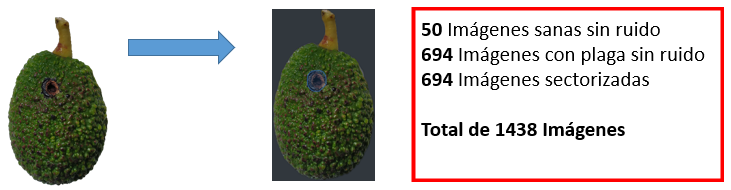
\includegraphics[width=0.7\textwidth]{resultados/proSeg.png}
\caption*{\footnotesize Fuente: Elaboración Propia}
\label{fig:figuraProSeg}
\end{figure}

Posteriormente se utilizó la aplicación DataTorch para hacer el trazado de los polígonos, en donde se coge una por una de las imágenes y se empieza a trazar cada una de las áreas en que se expresa la plaga, teniendo en cuenta que se hizo por cada una de las 694 imágenes dando un total de 1.438 imágenes, que incluye las imágenes sanas, las imágenes con plagas y las imágenes con los polígonos.

\begin{figure}[h]
\centering
\caption{Proceso de segmentación de las imágenes con DataTorch}
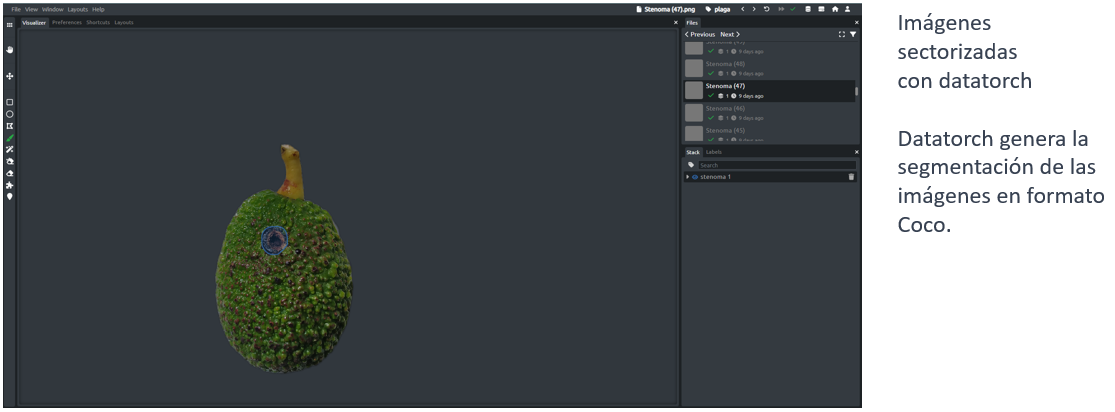
\includegraphics[width=0.7\textwidth]{resultados/proSeg2.png}
\caption*{\footnotesize Fuente: Elaboración Propia}
\label{fig:figuraProSegDatatorch}
\end{figure}

\subsubsection{Conjunto de entrenamiento y prueba}

El proceso de entrenamiento en Machine Learning implica enseñar a un modelo a reconocer patrones y tomar decisiones basadas en datos. Para lograr esto, es necesario dividir el conjunto de datos normalmente en dos partes: la primera, conocida como conjunto de entrenamiento, se utiliza para alimentar al modelo con ejemplos que le permitan aprender patrones y relaciones entre variables. Esta fase busca ajustar los parámetros del modelo para que pueda generalizar y hacer predicciones precisas sobre datos no vistos anteriormente.

\newpage

La segunda parte es el conjunto de validación, que actúa como una evaluación independiente del rendimiento del modelo. Al utilizar datos que el modelo no ha visto durante el entrenamiento, se puede evaluar su capacidad y prevenir problemas como el sobreajuste, donde el modelo memoriza los datos de entrenamiento en lugar de aprender patrones generales.

Dividir el conjunto de datos de las imágenes con plaga en conjuntos de entrenamiento y prueba como se describe a continuación:

\begin{figure}[h]
\centering
\caption{Proceso de entrenamiento y validación}
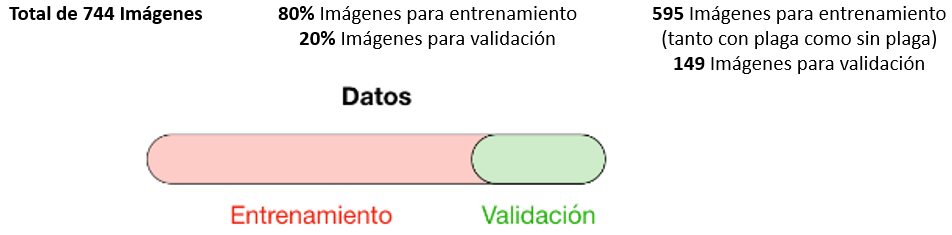
\includegraphics[width=1\textwidth]{resultados/proEntrenamiento.png}
\caption*{\footnotesize Fuente: Elaboración Propia}
\label{fig:figuraProEntrenamiento}
\end{figure}

Esta división en conjuntos de entrenamiento y validación es crucial para garantizar que el modelo pueda adaptarse a nuevos datos de manera efectiva, lo que mejora su capacidad predictiva y su utilidad en situaciones del mundo real.

Como para esta investigación se tiene un conjunto de datos moderado, es posible manejar un entrenamiento del de un 80/20; eso quiere decir que, del total de las imágenes 595 irán para el entrenamiento y 149 para validación, tanto la información con plaga como sin plaga, es decir se tiene toda la información conjunta.

Cabe señalar que existen otros porcentajes para el conjunto de datos como el 70/30 refiriéndose a 70\% entrenamiento y 30\% de validación, pero estos porcentajes son más útiles en conjuntos de datos más pequeños.

\subsection{Modelo de Machine Learning utilizando técnicas apropiadas de preprocesamiento y selección de características, así como algoritmos de aprendizaje supervisado o no supervisado, para lograr una detección de las plagas Stenoma catenifer y heilipus lauri en el cultivo de aguacate Hass}

\newpage

\subsubsection{Selección de algoritmos}

Para el proyecto se seleccionan algoritmos de aprendizaje supervisado o no supervisado adecuados para el problema de detección de plagas. Se seleccionó el algoritmo de la regresión logística, que es un algoritmo de clasificación que ayuda a determinar la probabilidad de que una imagen tenga o no tenga un objeto en este caso una plaga. El proceso corresponde a clasificar de manera binaria, entre cero y uno, donde cero es que no tiene plaga y el objeto uno donde sí tiene plaga.

También, se seleccionó el algoritmo de Yolo V8, que sus siglas en ingles significan You Only Look Once. Este algoritmo emplea redes neuronales convolucionales, estamos hablando de Deep learning, para facilitar e interpretar las imágenes. Este enfoque se integra en la fase de pre-procesamiento que se encarga de resaltar la zona afectada por la plaga, simplificando la tarea del algoritmo de Machine Learning y mejorando su capacidad de interpretación.

Estas redes neuronales convolucionales pueden aprender patrones y características complejas, permitiendo la identificación precisa de plagas en imágenes agrícolas. Además, el Deep Learning facilita la interpretación de las imágenes al automatizar la extracción de características, eliminando la necesidad de diseñar manualmente algoritmos específicos.

Para \cite{schmidhuber2015deep}, la capacidad del Deep Learning para adaptarse a patrones variados en imágenes, aprende automáticamente, agrupan gran cantidad de información, predicen comportamiento, los cuales contribuyen significativamente a mejorar la eficiencia y precisión en la detección de plagas. Su habilidad para generalizar a partir de conjuntos de datos grandes y diversos lo convierte en una herramienta poderosa para interpretar imágenes, proporcionando una base sólida para aplicaciones prácticas en la identificación y monitoreo de plagas, lo que en última instancia beneficia la gestión y la seguridad del proceso del cultivo de aguacate Hass.

\newpage

\begin{figure}[h]
\centering
\caption{Acción del algoritmo Yolo V8}
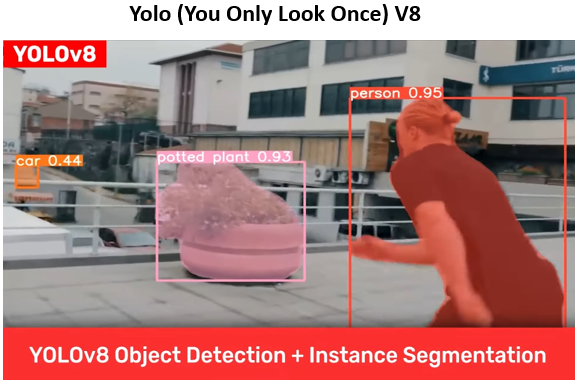
\includegraphics[width=0.7\textwidth]{resultados/yoloV8.png}
\caption*{\footnotesize Fuente: \cite{decoder2023}}
\label{fig:figuraYoloV8}
\end{figure}

En la imagen se puede ver que se clasifica un objeto con un 95\% de probabilidad de que sea una persona, un 93\% de establecer el objeto como “planta” y el otro objeto que se ve corresponde a un 44\% que el objeto sea un “carro”. El algoritmo Yolo V8 incluso puede ser usado en video, permitiendo en este caso detectar objetos incluso en tiempo real.

La selección del algoritmo de regresión logística se da porque es uno de los estándares para trabajar clasificación de imágenes en la industria. Por otro lado, el algoritmo Yolo es un algoritmo de Deep learning, para detectar objetos en imágenes esto se hace para determinar con una probabilidad de qué objetos se tienen en una imagen o imágenes e incluso en videos, siendo posible clasificar cada objeto que se encuentra en una imagen o video.

\subsubsection{Pre-procesamiento adicional}

El pre-procesamiento adicional correspondió a normalizar el tamaño de las imágenes. Esta acción fue necesaria debido a que permite trabajar con modelos de aprendizaje automático, como la regresión logística y Yolo. Esto se hace con el fin de reducir la complejidad computacional porque al tener imágenes de una resolución muy alta se va a requerir más procesamiento de cómputo para empezar a analizar pixel por pixel; a su vez ayuda a tener una consistencia en la entrada del modelo, porque todos los valores o variables del entrenamiento tendrán las mismas dimensiones y así se evitan problemas relacionados con la variabilidad que se puedan tener en el tamaño de las imágenes.

También habrá una normalización del modelo con datos nuevos, es decir que, si es necesario ingresar datos nuevos al modelo, pasaran por esta normalización cada uno de los datos en una resolución determinada.

Para la normalización de las dimensiones se definió un tamaño fijo de 640 píxeles, tanto de ancho como de alto, debido a que Yolo en su versión 8 maneja valores por defecto en esta resolución. Por esta razón, se mantuvo la misma resolución en los dos modelos seleccionados, tanto para el Yolo, que ya tiene por defecto este valor, como en la regresión logística. El siguiente código hace referencia a la normalización del tamaño de las imágenes, pero únicamente para el modelo de regresión logística, debido a que Yolo internamente hace esta normalización.

\begin{figure}[h]
\centering
\caption{normalización de las imágenes para la regresión logística}
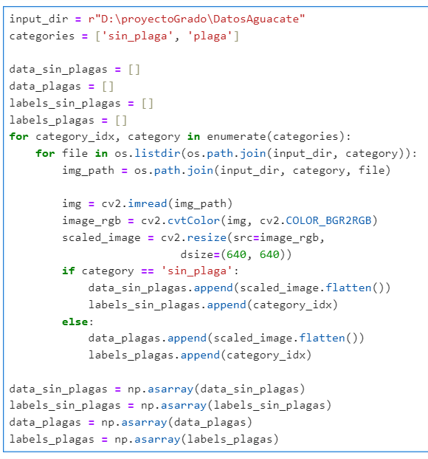
\includegraphics[width=0.6\textwidth]{resultados/normRegresion.png}
\caption*{\footnotesize Fuente: Elaboración Propia}
\label{fig:figuraNormRegresion}
\end{figure}

\newpage

\subsubsection{Implementación del modelo de regresión logística}

Para realizar la implementación del modelo de regresión logística, se realizó un balanceo de la información debido a la disparidad entre los datos con plagas (694), de los datos sanos (50). De allí que, se implementó un balanceo de información hacia abajo, es decir que la clase mayoritaria se tiene que igualar a su clase minoritaria para poder hacer comparaciones y hacer un entrenamiento más proporcional con la información.

\begin{figure}[h]
\centering
\caption{proceso de normalización de imágenes}
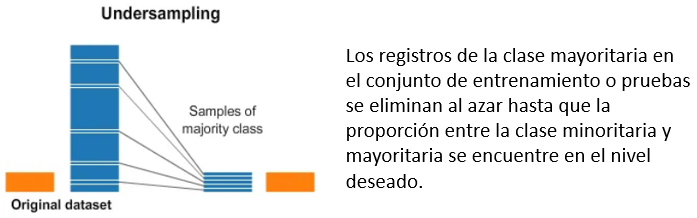
\includegraphics[width=0.8\textwidth]{resultados/proNormalizacion.png}
\caption*{\footnotesize Fuente: Elaboración Propia}
\label{fig:figuraProNormalizacion}
\end{figure}

Se realizó un submuestreo con validación cruzada (cross-validated subsampling). En este enfoque, se realiza repetidamente un submuestreo de la clase mayoritaria para equilibrar las clases y se evalúa el modelo en cada iteración utilizando la clase minoritaria. Luego, se promedian los resultados obtenidos en todas las iteraciones.

Este enfoque es especialmente útil cuando se trata con conjuntos de datos desequilibrados, donde una clase tiene muchas más datos (imágenes) que otra. Al realizar varias iteraciones y calcular promedios, se busca obtener una evaluación más robusta del rendimiento del modelo, ya que cada iteración puede tener una muestra diferente de la clase mayoritaria.

En el desarrollo de los scripts para implementar el modelo de regresión logística se realizan los siguientes pasos:

\newpage

\begin{enumerate}
    \item Se va a repetir el proceso de entrenamiento y evaluación 10 veces.
    \item Se realiza el balanceo de los datos en la clase mayoritaria (con plagas) sacando subconjuntos aleatorios de 50 imágenes del conjunto total (694).
    \item Se combinan los datos de 'sin plaga' y datos balanceados de 'plaga’ para tener un subconjunto de 100 imágenes totales 50 sin plaga y 50 con plaga.
    \item Se dividen los datos en conjuntos de entrenamiento y prueba en 80/20, es decir, 80 imágenes de entrenamiento y 20 imágenes para prueba.
    \item Se inicializa el modelo de regresión logística con la dependencia sklearn.
    \item Se pasa a entrenar el modelo con los subconjuntos de entrenamiento.
    \item Se realizan las predicciones en los subconjuntos de prueba.
    \item Se calcula la matriz de confusión y se almacena por cada subconjunto.
    \item Se calcula el promedio de las exactitudes (accuracy) obtenidas desde las matrices de confusión.
    \item Se calcula el promedio de las precisiones obtenidas desde las matrices de confusión.
    \item Se calcula el promedio de las sensibilidades (recall) obtenidas desde las matrices de confusión.
\end{enumerate}

\newpage

\begin{figure}[h]
\centering
\caption{Código desarrollado para el modelo de regresión logística}
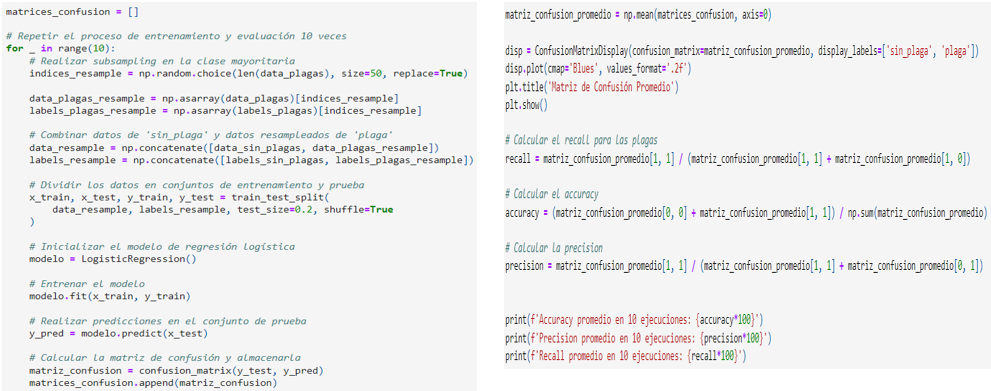
\includegraphics[width=1\textwidth]{resultados/codModelRegresion.png}
\caption*{\footnotesize Fuente: Elaboración Propia}
\label{fig:figuraCodModelRegresion}
\end{figure}

Para el desarrollo de los scripts que implementan el modelo Yolo V8 se realizaron los siguientes pasos:

\begin{enumerate}
    \item Se establece que se van a manejar por convención del modelo Yolo, dos particiones (entrenamiento – train y validación – validation) (ver figura \ref{fig:figuraConvencionYolo}).
    \item Se dividen los datos en las particiones de entrenamiento y prueba en 80\%/20\% de 744 imágenes, es decir, 595 imágenes de entrenamiento y 149 imágenes para prueba.
    \item Se realiza la transformación del formato Coco al formato Yolo para cada imagen  (ver figura \ref{fig:figuraCocoAYolo})\footnote{Se realiza la transformación del formato Coco para cada imagen al formato Yolo, porque en el objetivo uno la segmentación de imágenes se realizó con la herramienta DataTorch la cual utiliza el formato Coco para generar las anotaciones correspondientes en las imágenes, pero el algoritmo Yolo solo funciona con el formato Yolo.}.
    \item Se escribe en un archivo de texto la transformación del formato resultante.
    \item Se copia el archivo en la partición correspondiente (entrenamiento o prueba).
    \item Se importa la dependencia para trabajar con Yolo (ultralytics).
    \item Se establece el modelo a Yolo small \footnote{Yolo en su versión 8 salió en enero del año de 2023 y presenta diferentes modelos para diferentes tareas teniendo en cuenta las necesidades para detectar o segmentar información. Para esta investigación se manejó el modelo correspondiente a la detección de objetos. Para saber más sobre los diferentes tipos de modelos, se puede encontrar información detallada en el enlace \href{https://docs.ultralytics.com/es/models/yolov8/\#tareas-y-modos-compatibles}{tipos de modelos Yolo}. }. 
    \item Se establecen 10 épocas para correr el modelo.
    \item Se obtienen los resultados arrojados por el algoritmo (predicciones y sensibilidades - recall).
\end{enumerate}

El concepto de ``épocas'' se refiere a la cantidad de veces que todo el conjunto de datos se ha pasado hacia adelante y hacia atrás a través de la red neuronal durante el proceso de entrenamiento. Cada época representa una iteración completa a través de todo el conjunto de datos.
Manejar múltiples épocas durante el entrenamiento puede tener varios beneficios:

\textbf{Aprendizaje más Profundo:}

Las redes neuronales, incluidas las arquitecturas complejas como YOLO, pueden aprender patrones más profundos y sutiles a medida que se exponen repetidamente a los datos. Las épocas adicionales permiten que el modelo ajuste sus pesos en consecuencia y mejore su capacidad para generalizar a patrones más complejos.

\textbf{Mejora de la Generalización:}

El entrenamiento con más épocas puede ayudar a mejorar la capacidad del modelo para generalizar a datos no vistos. Esto es particularmente útil para evitar el sobreajuste, donde el modelo memoriza los datos de entrenamiento en lugar de aprender patrones, ubicaciones o lugares generales.

\textbf{Ajuste Fino de Parámetros:}

Las épocas adicionales permiten ajustar finamente los parámetros del modelo. A medida que el modelo ve los datos varias veces, puede hacer ajustes más precisos en los pesos para mejorar el rendimiento en el conjunto de entrenamiento.

\textbf{Mejora de Métricas de Rendimiento:}

En muchos casos, las métricas de rendimiento (como precisión, recall, F1-score, etc.) pueden mejorar con un entrenamiento más prolongado. Las métricas estabilizan y pueden alcanzar su mejor rendimiento después de varias épocas.

\newpage

Manejar 10 épocas podría ser mejor que manejar pocas épocas, esto puede depender de la complejidad del problema, del tamaño del conjunto de datos y de la arquitectura específica del modelo. Más épocas generalmente significan más oportunidades para que el modelo aprenda y mejore, siempre y cuando se evite el sobreajuste. Sin embargo, no siempre es necesario o beneficioso utilizar un gran número de épocas, ya que podría aumentar los costos computacionales sin proporcionar mejoras significativas en el rendimiento del modelo.

\begin{figure}[h]
\centering
\caption{Código convención del modelo Yolo}
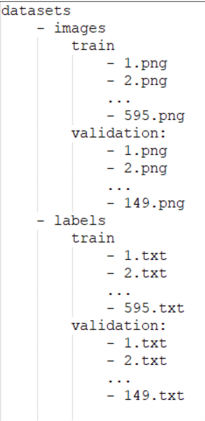
\includegraphics[width=0.2\textwidth]{resultados/convencionYolo.png}
\caption*{\footnotesize Fuente: Elaboración Propia}
\label{fig:figuraConvencionYolo}
\end{figure}

\begin{figure}[h]
\centering
\caption{Código transformación de formato Coco a formato Yolo}
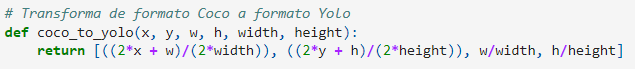
\includegraphics[width=0.8\textwidth]{resultados/cocoAYolo.png}
\caption*{\footnotesize Fuente: Elaboración Propia}
\label{fig:figuraCocoAYolo}
\end{figure}

\newpage

Dentro del código anterior se especifica el cambio del formato Coco a Yolo partiendo de las categorías establecidas con la plaga y si no tiene plaga no se denota. Como se describe en el código se escribe las dimensiones de ancho y alto para las anotaciones, donde dice que para una imagen dentro del polígono se encuentra la plaga denotada en los cuatro lados expresados en cuatro valores (x, y, w, h) que son la coordenada X y Y en donde se ubica el extremo superior del polígono a marcar, como el ancho y alto en donde se encuentra la placa.

Estos parámetros de la cooredanada X y Y del polígono en formato Yolo, se posicionan en el centro de la imagen donde está ubicado el objeto, en este caso se mueve a su centro, y esto se hace con una fórmula matemática  como se observa en la siguiente imagen:


\begin{figure}[h]
\centering
\caption{Proceso de cambio de Coco a Yolo}
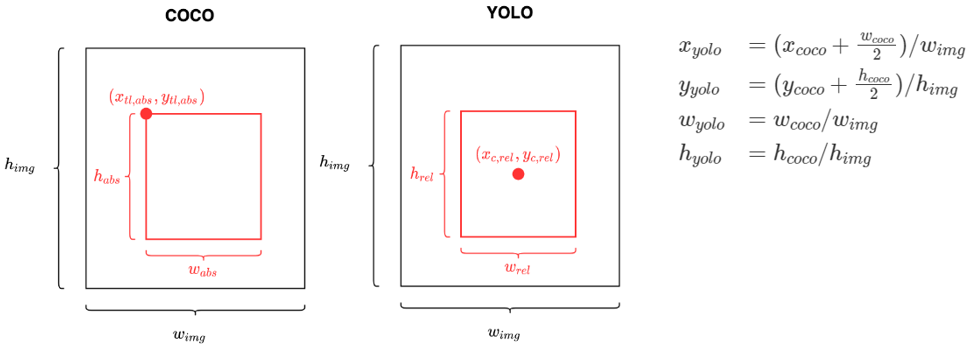
\includegraphics[width=1\textwidth]{resultados/camCocoAYolo.png}
\caption*{\footnotesize Fuente: Elaboración Propia}
\label{fig:figuraCamCocoAYolo}
\end{figure}

Después de realizar la transformación, el procedimiento implica identificar y organizar la información (ver figura \ref{fig:figuraPoligonoCocoAYolo}) de la siguiente manera:
\begin{itemize}
    \item La primera columna especifica la clase a utilizar, en este caso, ``plaga'' \footnote{La acción matemática es descrita en \cite{rehman2022conversion} especificando los procedimientos para el cambio de Coco a Yolo.}. 
    \item La segunda y tercera columna indican las coordenadas del punto medio de un cuadro delimitador, correspondiente a la posición central del objeto a identificar, en este caso, la plaga. 
    \item La cuarta y quinta columna contienen las dimensiones del cuadro delimitador, representando respectivamente el ancho y alto del objeto en cuestión. Para clarificar. la cuarta columna representa el ancho, mientras que la quinta columna refleja el alto. Este proceso se aplica para facilitar la identificación y delimitación de la plaga.
\end{itemize}

\begin{figure}[h]
\centering
\caption{Identificación del polígono cambiado de Coco a Yolo}
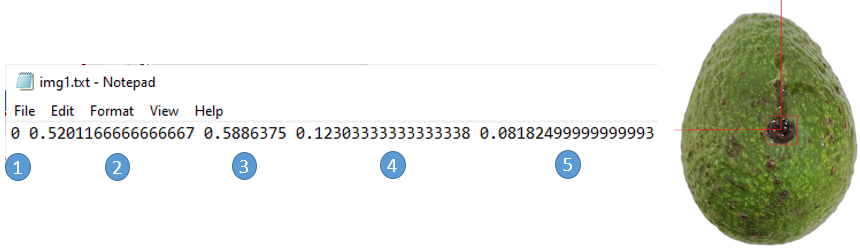
\includegraphics[width=1\textwidth]{resultados/poligonoCocoAYolo.png}
\caption*{\footnotesize Fuente: Elaboración Propia}
\label{fig:figuraPoligonoCocoAYolo}
\end{figure}


Este proceso corresponde a la conversión del formato Coco a Yolo. En otras palabras, se especifica una clase, en este caso, ``plaga'' designada como cero. Los dos primeros valores indican las coordenadas del punto medio del cuadro que se va a delimitar, mientras que los dos valores restantes representan el alto y el ancho de la imagen en cuestión. Este código pertenece al modelo Yolo V8, donde se lleva a cabo la distribución de las imágenes en las dos particiones correspondientes de entrenamiento y validación.


\subsubsection{Implementación del modelo Yolo}

La siguiente imagen \ref{fig:figuraCodModelYolo} hace referencia a la implementación para el modelo Yolo. En donde:

\begin{itemize}
    \item Los puntos 1 y 2 hacen referencia al preprocesamiento que se le van a aplicar a las imágenes para el modelo Yolo.
    \item El punto 3 se observa que se carga el modelo en el código Yolo V8 en su versión small, definiendo las épocas, en este caso 10, las cuales van a procesar la información, teniendo en cuenta que entre más épocas mayor es el costo computacional para obtener un resultado. 
\end{itemize}

\newpage

\begin{figure}[h]
\centering
\caption{Código desarrollado para el modelo Yolo V8}
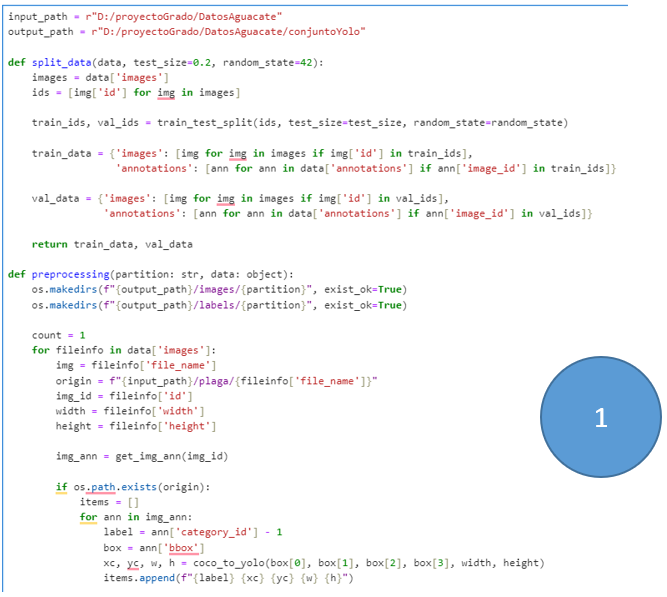
\includegraphics[width=0.4\textwidth]{resultados/codModelYoloP1.png}
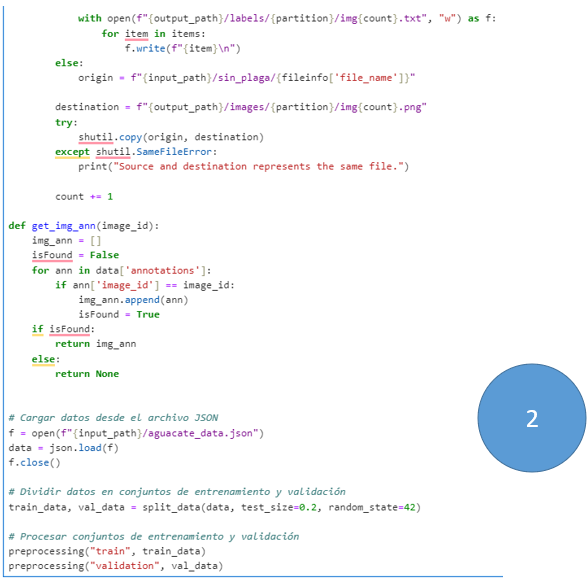
\includegraphics[width=0.4\textwidth]{resultados/codModelYoloP2.png}
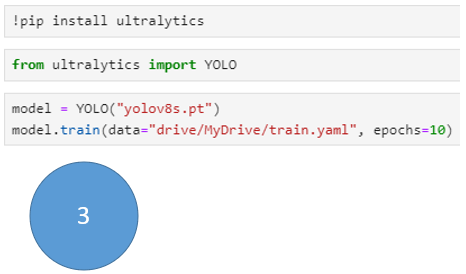
\includegraphics[width=0.4\textwidth]{resultados/codModelYoloP3.png}
\caption*{\footnotesize Fuente: Elaboración Propia}
\label{fig:figuraCodModelYolo}
\end{figure}

\subsubsection{Evaluación de los modelos}

Después de haber entrenado los modelos y pasar a predecir la información que se tenga del  conjunto de prueba, es decir identificar qué tanto aprendió y cuál fue el porcentaje de aprendizaje que se tuvo, para ambos casos se manejó una matriz de confusión donde se tienen cuatro lados: falso positivo, falso negativo, verdadero negativo, verdadero positivo (ver figura \ref{fig:figuraEvaModelos}).

\newpage

\begin{figure}[h]
\centering
\caption{Matriz de confusión para la evaluación de los modelos}
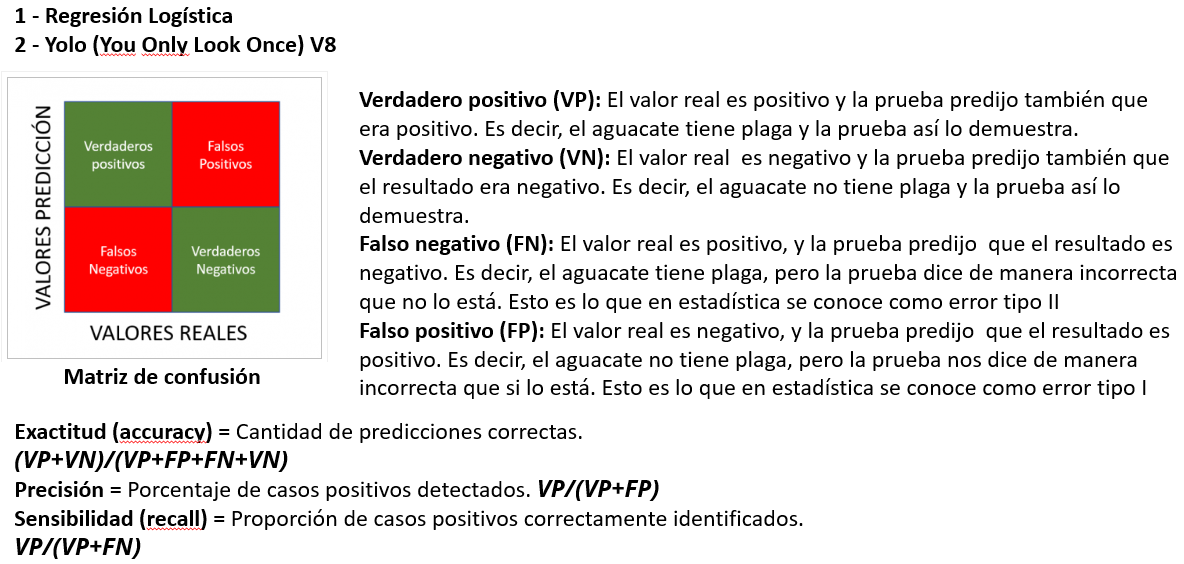
\includegraphics[width=1\textwidth]{resultados/evaModelos.png}
\caption*{\footnotesize Fuente: Elaboración Propia}
\label{fig:figuraEvaModelos}
\end{figure}

Una interpretación efectiva de la matriz de confusión en un modelo Yolo es esencial para entender cómo se comporta en términos de identificación y ubicación de objetos en las imágenes de entrada. Al analizar los elementos de la matriz, los científicos de datos pueden ajustar el modelo para mejorar su rendimiento y garantizar una detección precisa de objetos en diferentes escenarios y condiciones.

Para la regresión logística al tener 10 iteraciones se calculó el promedio de esas matrices de confusión, es decir que cada vez que se pasaba el modelo en este subconjunto de datos de 100 imágenes se estaba calculando una matriz de confusión, se van guardando cada una de esas matrices y al final lo que se hace es promediarlas, para tener los resultados de exactitud, precisión y sensibilidad como se describe en la imagen \ref{fig:figuraEjeProMatrizConfusion}.


\newpage

\begin{figure}[h]
\centering
\caption{Resultado promedio de la matriz de confusión del modelo de regresión}
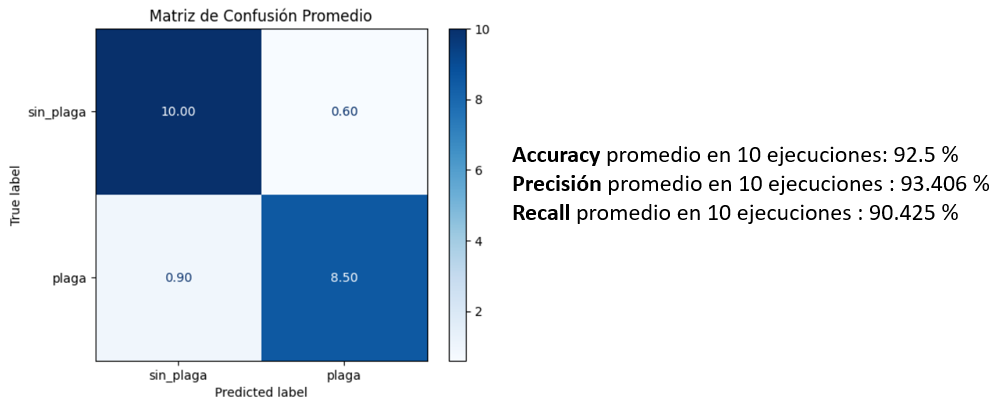
\includegraphics[width=1\textwidth]{resultados/ejeProMatrizConfusion.png}
\caption*{\footnotesize Fuente: Elaboración Propia}
\label{fig:figuraEjeProMatrizConfusion}
\end{figure}

El objetivo es determinar la cantidad de datos que estaban etiquetados como afectados por una plaga durante la prueba del modelo. En este escenario, se utiliza un subconjunto de 100 imágenes para llevar a cabo las pruebas, y se espera que dicho subconjunto represente un porcentaje específico del total correspondiente al 20\% para las pruehas.

Además, la parte de evaluación del modelo de regresión logística, después de haber hecho las iteraciones de la información para entrenar el modelo, en cada iteración se fue almacenando su matriz de confusión. Este proceso obtiene la matriz de confusión de cada uno de las iteraciones, las cuales se promedian y se obtienen el cálculo de la exactitud (accuracy), la precisión y la sensibilidad (recall), como se describe en el código de la imagen \ref{fig:figuraCodEvaModelRegresion}. 

Entonces eso quiere decir que cuando se habla de precisión se especifica la cantidad de casos positivos detectados, lo que significa que para este caso fueron realmente positivos detectados en un 93.4\%, una sensibilidad que corresponde a la proporción de los casos positivos correctamente identificados que fue de un 90.4\%. Para el caso de la exactitud se evidenció un 92.5\%, es decir la cantidad de predicciones correctas esta en este porcentaje, siendo un buen promedio de predicción para validar si una imagen tiene o no tiene plaga en un 92.5\%.

\newpage

\begin{figure}[h]
\centering
\caption{Código evaluación del modelo utilizando regresión logística en el conjunto de prueba.}
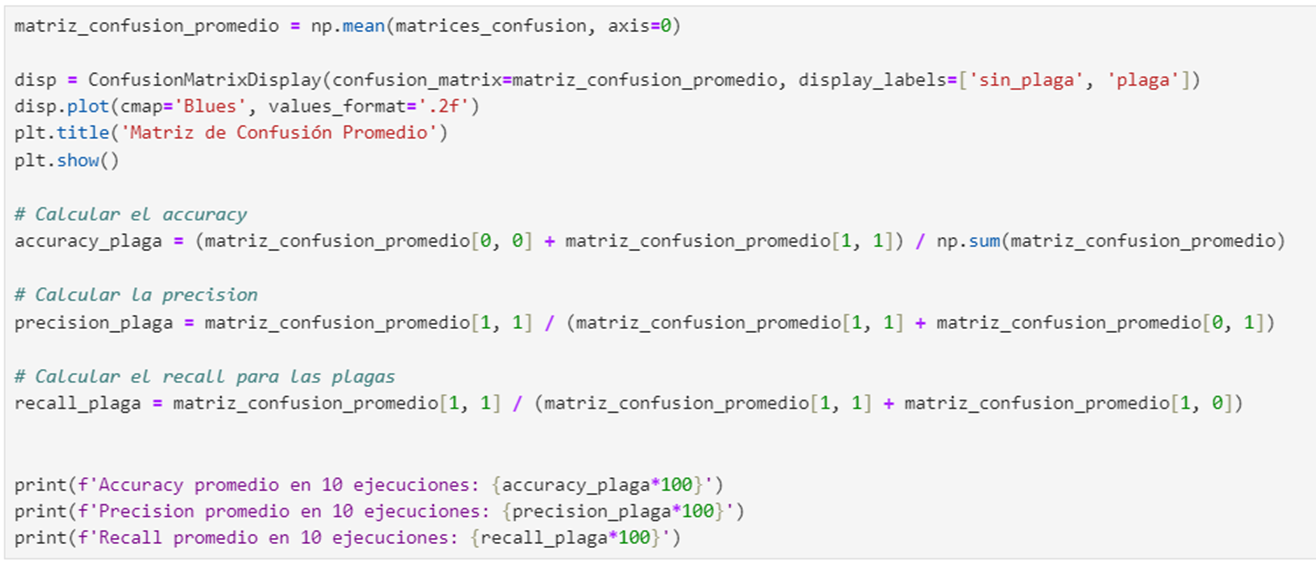
\includegraphics[width=1\textwidth]{resultados/codEvaModelRegresion.png}
\caption*{\footnotesize Fuente: Elaboración Propia}
\label{fig:figuraCodEvaModelRegresion}
\end{figure}

Si se volviera a ejecutar el programa, es posible que la información varíe ligeramente, pero en términos generales, los resultados que se presentan corresponden a la ejecución más reciente del algoritmo. Es importante destacar que las variaciones observadas en la exactitud, la precisión y la sensibilidad son mínimas. Estas fluctuaciones, aunque pueden existir cambios sutiles, la diferencia no es significativa.

En Yolo V8, ya no es necesario clasificar las imágenes que no contienen plagas. Ahora, el enfoque se centra únicamente en clasificar las imágenes que efectivamente presentan plagas. Cuando se procesa la información que carece de plagas, el algoritmo simplemente ignora o descarta dicha información, ya que el objetivo principal consiste en identificar si una imagen específica del conjunto de prueba contiene o no una subimagen, polígono o recuadro que pueda representar una plaga. En otras palabras, el propósito es determinar si dentro de la representación visual de un aguacate existe o no la presencia de una plaga. El enfoque se ha optimizado para dirigir la atención exclusivamente a las instancias relevantes, simplificando el proceso de clasificación y mejorando la eficiencia del modelo.


\newpage

\begin{figure}[h]
\centering
\caption{Resultado del modelo Yolo V8}
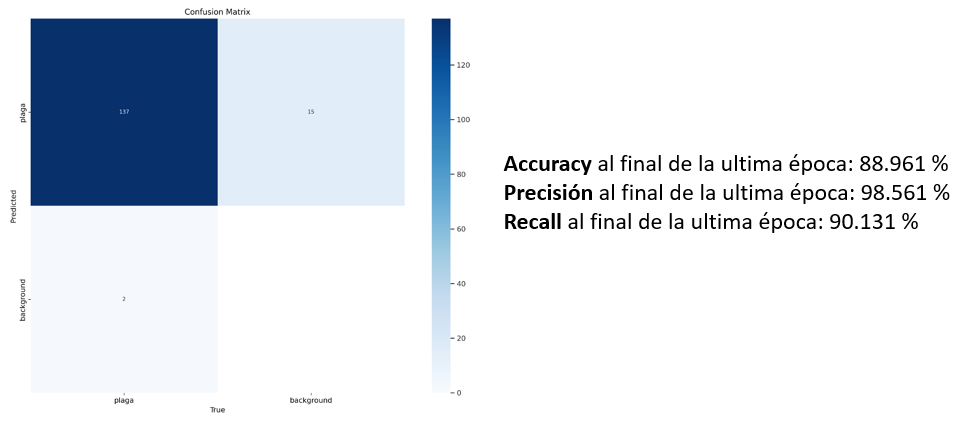
\includegraphics[width=1\textwidth]{resultados/ejeProMatrizConfusionYolo.png}
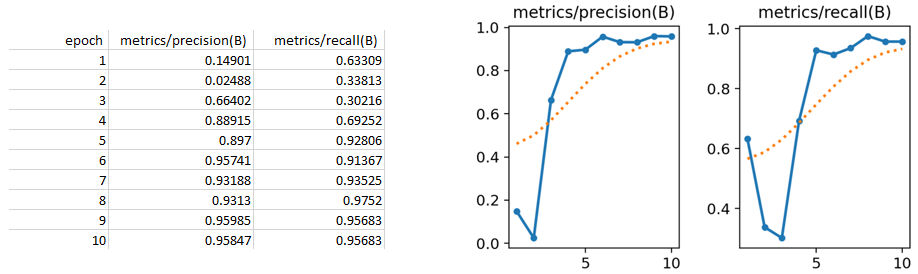
\includegraphics[width=1\textwidth]{resultados/resYolo.png}
\caption*{\footnotesize Fuente: Elaboración Propia}
\label{fig:figuraEjeProMatrizConfusion}
\end{figure}

Después de realizar la evaluación, observamos que la sensibilidad (recall) alcanzó un 90\%, indicando que el 90\% de los casos positivos fueron correctamente identificados respecto al total de imágenes. La precisión, que mide la proporción de casos positivos correctamente detectados entre las predicciones positivas, se situó en un sólido 98\%. Por otro lado, la exactitud (accuracy), que representa la cantidad general de predicciones correctas, se registró en un 88\%. Esto implica que, aunque se logró una alta precisión, hubo algunas predicciones incorrectas, especialmente en casos específicos evaluados por el modelo Yolo.


\newpage

Es importante destacar que la evaluación se llevó a cabo con imágenes que tenian y carecían de plagas, es decir, imágenes consideradas como ``sanas''. Además, es relevante señalar que la matriz de confusión se generó de manera automática, proporcionando una representación visual detallada de los resultados de la evaluación.

Yolo genera imágenes y proporciona métricas clave como precisión, recall y curvas de aprendizaje por época. Al analizar las estadísticas por época, se observa una progresión significativa en la precisión a lo largo del entrenamiento. En las primeras épocas, la precisión fue baja, alcanzando solo el 14.1\% en la primera y el 2\% en la segunda. Sin embargo, a partir de la tercera época, se observa un aumento marcado, llegando al 66\% en la época 6 y alcanzando un impresionante 95\% en la época 7. Las épocas 8, 9 y 10 mantienen rendimientos destacados, con la época 9 mostrando una precisión aún mayor que la 10 (ver figura \ref{fig:figuraEjeProMatrizConfusion}).

El análisis detallado revela que, a pesar de obtener altos valores de recall, la precisión disminuyó en la época 10, este análisis subraya la importancia de equilibrar la precisión y el recall al ajustar el número de épocas. La representación gráfica destaca cómo el modelo evoluciona en cada época, evidenciando mejoras notables a partir de la quinta época. La tabla complementa visualmente la información proporcionando valores precisos de precisión y recall para cada época. En retrospectiva, la decisión de detener el entrenamiento en la época 9 podría haber resultado en un rendimiento óptimo, ya que se logró una alta precisión sin comprometer significativamente el recall. Este análisis proporciona valiosas percepciones para optimizar futuros entrenamientos del modelo Yolo.

En los resultados proporcionados por el modelo, se presentan imágenes que fueron clasificadas como casos de plagas. Al analizar estas imágenes, es evidente que el modelo ha identificado correctamente la presencia de plagas, ya que estas son las mismas imágenes que proporcioné individualmente al algoritmo para su evaluación. En el conjunto de prueba generado, las representaciones visuales de plagas son claramente evidentes en las imágenes que se muestran en el lado derecho. Estas imágenes son el resultado de la aplicación del algoritmo, demostrando su capacidad para discernir y clasificar eficazmente las instancias de plagas en base a los patrones aprendidos durante el entrenamiento.

\newpage

\begin{figure}[h]
\centering
\caption{Visualización de la evaluación realizada con Yolo V8}
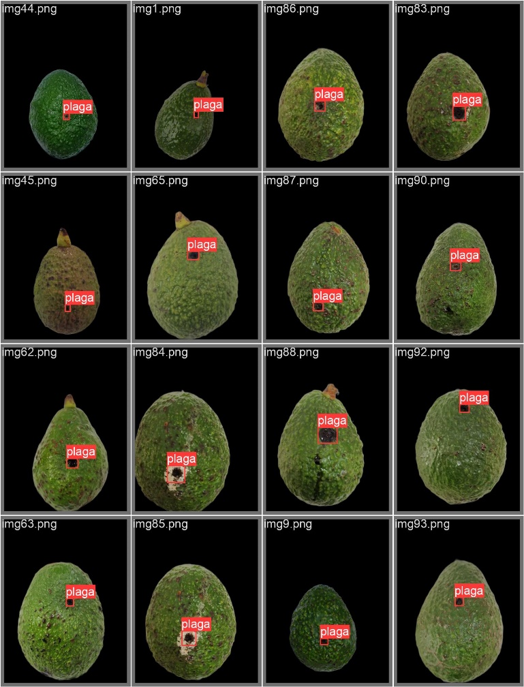
\includegraphics[width=1\textwidth]{resultados/visPruebasYolo.png}
\caption*{\footnotesize Fuente: Elaboración Propia}
\label{fig:figuraVisPruebasYolo}
\end{figure}

Este conjunto de resultados subraya la eficacia del modelo Yolo en la tarea específica de identificación de plagas, respaldando la calidad de las predicciones al compararlas con la evaluación visual que se realizó de manera automática. La capacidad del algoritmo para generalizar y reconocer patrones de plagas en nuevas imágenes es un indicativo positivo de su rendimiento y validez en aplicaciones prácticas relacionadas con la detección y clasificación de problemas específicos, como la presencia de plagas en cultivos.

Al evaluar el desempeño del algoritmo Yolo V8 en la validación de imágenes de plagas, se destaca la efectividad de la detección. En el conjunto de validación, el algoritmo demuestra su capacidad para identificar plagas en imágenes específicas sin conocer previamente la ubicación de los polígonos anotados. La separación del conjunto de datos en entrenamiento y prueba es esencial, y el conjunto de validación, con un 20\% de las imágenes, se utiliza para evaluar el rendimiento del modelo.

\newpage

Las imágenes seleccionadas para la validación no siguen un orden específico y son elegidas al azar por el algoritmo. Al analizar las imágenes detectadas, el algoritmo asigna porcentajes de confianza para cada región identificada como plaga, facilitando la interpretación de la certeza de las predicciones. Se observa que el algoritmo genera predicciones de plagas con confianza superior al 70\%.

La potencial aplicación práctica del modelo se ilustra al considerar su capacidad para clasificar imágenes en tiempo real, incluso mediante el análisis de videos. Esta capacidad permite no solo la detección de plagas, sino también la visualización gráfica instantánea de las áreas afectadas. La versatilidad del modelo Yolo V8 corresponde al poder aplicarse en situaciones dinámicas y en tiempo real.